% Make nice A4 pages for print:
%\usepackage{pgfpages}
%\pgfpagesuselayout{resize to}[a4paper,border shrink=5mm,landscape]

\beamertemplatenavigationsymbolsempty

\setbeamertemplate{bibliography item}[text]

\usepackage[type={CC},modifier={by-sa},version={4.0}]{doclicense}

\usepackage[utf8]{inputenc}
\usepackage{hyperref}
\usepackage{breakurl}
\usepackage{graphicx}
\usepackage{pgfplots}
\usepackage{pgf}
\usepackage{tikz}
\usetikzlibrary{positioning}
\usetikzlibrary{arrows}
\usetikzlibrary{decorations.markings}
\usetikzlibrary{calc}
\usetikzlibrary{matrix}
\usetikzlibrary{shapes}
\usetikzlibrary{decorations.pathmorphing}
\usetikzlibrary{fit}
\usetikzlibrary{backgrounds}
\usetikzlibrary{plotmarks}
\usepackage{stmaryrd}
\usepackage{listings}
\usepackage{pdflscape}
\usepackage{perpage}
\usepackage{appendixnumberbeamer}

%\usepackage[thmmarks,amsmath,amsthm]{ntheorem} % already included in beamer
\usepackage{thm-restate}

\usepackage[sort&compress,numbers]{natbib}  % to be have \citet, \citeauthor, \citeyear

\MakePerPage{footnote}

\tikzstyle{o}=[r,ppBlue]
\tikzstyle{r}=[thick,rectangle,align=center]
\tikzstyle{t}=[r,ppTrans] %,font=\bfseries]
\tikzstyle{dd}=[densely dashed]
\tikzstyle{n}=[r,ppBlue]
\tikzstyle{p}=[r,ppRed]
\tikzstyle{ppRed}  =[draw=red,  fill=  red!20]
\tikzstyle{ppBlue} =[draw=blue, fill= blue!20]
\tikzstyle{ppGreen}=[draw=green,fill=green!20]
\tikzstyle{ppTrans}=[draw=none, fill=none]

\usetheme{Warsaw}

\useoutertheme[subsection=true]{smoothbars}
%\useoutertheme[subsection=false]{miniframes}

\definecolor{bblue}{HTML}{D7DF01}	% yellow-ish actually, for better black/white printing
\definecolor{rred}{HTML}{C0504D}
\definecolor{ggreen}{HTML}{9BBB59}
\definecolor{ppurple}{HTML}{9F4C7C}
\definecolor{lightgray}{rgb}{0.3,0.3,0.3}
\definecolor{lightergray}{rgb}{0.9,0.9,0.9}
\definecolor{UniBlue}{RGB}{83,121,170}

\DeclareTextFontCommand\textintro{\normalfont\bfseries\itshape} % nice!
\newcommand{\intro}[2][]
{%
	\textintro{#2}%
}
\newcommand{\empha}[2][]
{%
	\emph{#2}%
}

%\theoremstyle{plain}
\newcounter{reqcounter}
\newtheorem{requirement}[reqcounter]{Requirement}

%setbeamercolor{structure}{fg=violet}

\makeatletter
\def\th@task{%
    \normalfont % body font
    \setbeamercolor{block title example}{bg=orange,fg=white}
    \setbeamercolor{block body example}{bg=orange!20,fg=black}
    \def\inserttheoremblockenv{exampleblock}
  }
\makeatother

\theoremstyle{task}
\newtheorem{task}{Task}

\newenvironment{assignment}%
{%\setbeamercolor{background canvas}{bg=violet}%
%\setbeamercolor{structure}{fg=cyan!90!black}%
 \setbeamercolor{frametitle}{bg=orange,fg=white}
\begin{frame}}%
{\end{frame}}%

\AtBeginSection[]{
  \begin{frame}
  \vfill
  \centering
  \begin{beamercolorbox}[sep=8pt,center,shadow=true,rounded=true]{title}
    \usebeamerfont{title}\insertsectionhead\par%
  \end{beamercolorbox}
  \tableofcontents
  \vfill
  \end{frame}
}




\pgfplotsset{compat=1.14}
\author{Markus Raab}


\date{1.6.2018}

\begin{document}

\renewcommand{\enquote}[1]{\emph{``#1''}} % Cannot be done earlier

%%%%%%%%%%%%%%%%%%%%%%%%%%%%%%%
\begin{frame}
	\titlepage
	\doclicenseThis
\end{frame}

\begin{frame}
	\frametitle{Organization}
	Schedule:
	\begin{description}
		\item[8.6.2018:] lecture
		\item[15.6.2018:] last corrections of team exercise
		\item[22.6.2018:] oral test
	\end{description}
\end{frame}


\begin{frame}
	\frametitle{Popular Topics}
	\vspace{-0.5cm}
	\begin{multicols}{2}
	\begin{description}
	\color{red}
	\item[4] validation
	\color{black}
	\item[4] user interface
	\color{gray}
	\item[3] tools (benefits?)
	\item[3] testability
	\item[3] complexity reduction (when conf. needed?)
	\item[3] architectural decisions
	\color{black}
	\item[2] Puppet
	\color{gray}
	\item[2] modularity
	\item[2] environment variables
	\color{gray}
	\item[2] documentation
	\color{red}
	\item[2] configuration specification
	\color{gray}
	\item[2] command-line args\color{black}
	\color{gray}
	\item[2] code generation
	\item[1] variability
	\color{red}
	\item[1] self-description
	\item[1] round-tripping
	\color{gray}
	\item[1] early detection
	\item[1] introspection
	\item[1] dependences
	\item[1] auto-detection
	\item[1] context-awareness
	\color{black}
	\item[1] administrators
	\end{description}
	\end{multicols}
\end{frame}

\begin{frame}
	\hspace*{-1cm}\includegraphics[width=\paperwidth]{dot/topics}
\end{frame}

\begin{frame}
	\frametitle{Introspection (Recapitulation)}
	\begin{task}
	What is internal and external specification?
	What is introspection?
	\end{task}

	\pause
	\vspace{1em}

	\begin{itemize}
	\item \textit{internal}: within applications' source code
	\item \textit{introspection}: unified get/set access to (meta*)-key/values
	\item access via applications, CLI, GUI, web-UI, ...
	\item access via any programming language (similar to file systems)
	\item GUI, web-UI can semantically interpret metadata
	\item assemble modular parts (validation, logging, \dots)
	\item needed as communication between producers and consumers
	\item essential for \intro[no-futz computing]{no-futz computing}~\citet{holland2001nofutz}
	\end{itemize}
\end{frame}

\begin{frame}
	\frametitle{KeySet (Recapitulation)}

	The common data structure of Elektra:
	\vspace{1cm}

	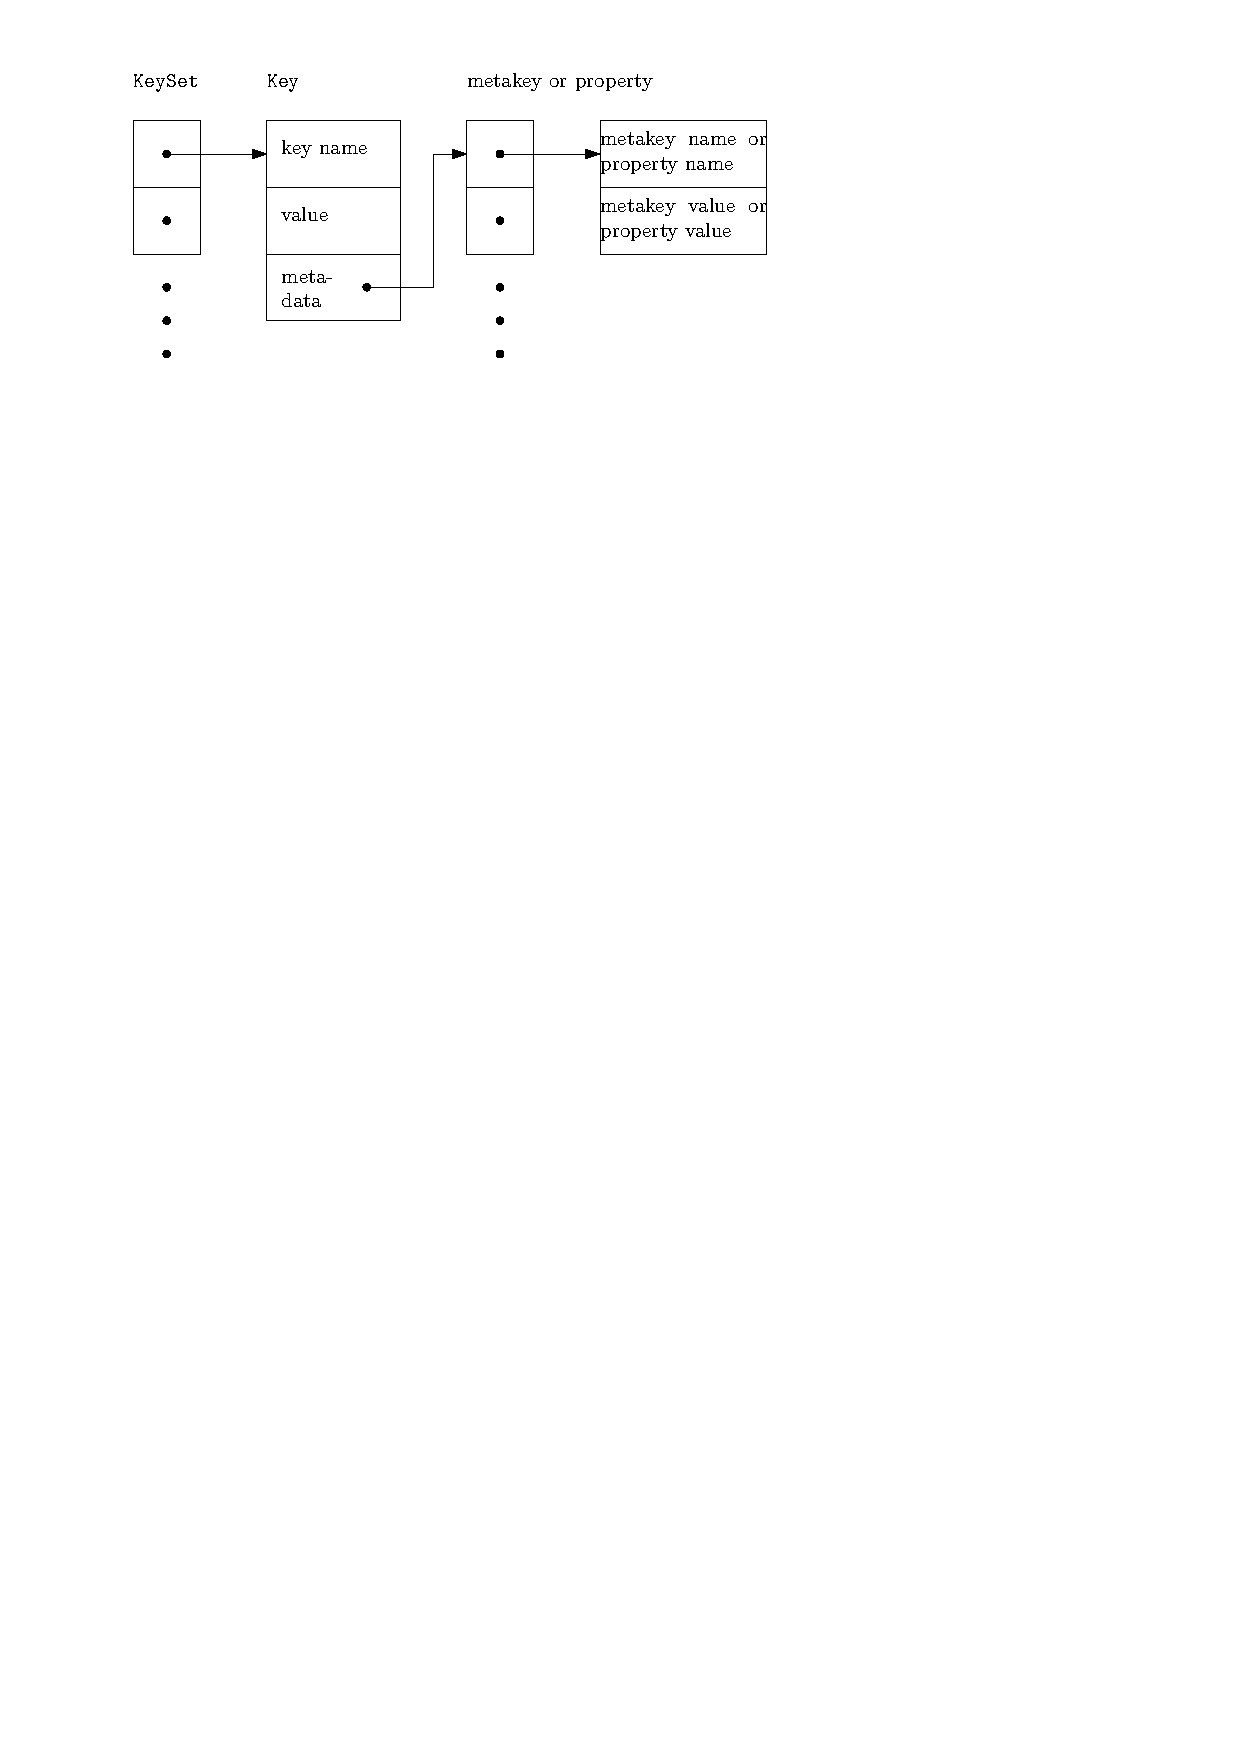
\includegraphics{keyset}
\end{frame}

\begin{frame}
	\frametitle{Testing (Recapitulation)}
	\begin{task}
	What do we want to test?
	\end{task}

	\pause

	\begin{itemize}
	\item That settings do what they should (devs and admins)
	\item That settings are properly validated (devs~\cite{xu2013blame})
	\item Regression tests (devs~\cite{qu2008configuration})
	\vspace{1em}
	\item Are all settings implemented? (devs)
	\item Are all settings used in tests? (devs)
	\item Are there unused settings in the code? (devs)
	\item Do the chosen settings work? (admins)
	\end{itemize}
\end{frame}

\begin{frame}
	\frametitle{Early detection (Recapitulation)}
	\begin{task}
	When do we want to detect misconfiguration?
	\end{task}

	\pause

	Phases when we can detect misconfigurations:
	\begin{itemize} %[<+-| alert@+>]
	\item Compilation stage in configuration management tool
	\item Writing configuration settings on nodes
	\item Starting applications (load-time)
	\item When configuration setting is actually used (run-time)
	\end{itemize}

	\pause[\thebeamerpauses]

	\begin{alertblock}{Problem}
	Earlier versus more context.
	\end{alertblock}
\end{frame}

\begin{frame}
	\frametitle{Notification (Recapitulation)}

	\begin{task}
	Why do we need notification?
	\end{task}

	\pause

	\begin{enumerate}
	\item to keep transient and persistent configuration settings always in sync~\cite{jin2014configurations}
	\item to avoid polling of configuration settings
	\item to better integrate into already existing mechanisms (main loops)\footnote{Is one of the main reasons why most framework already integrate configuration settings.}
	\end{enumerate}

	\ExecuteMetaData[../book/motivation.tex]{req-consistency}
\end{frame}

\begin{frame}
	\frametitle{Cascading (Recapitulation)}

	\begin{task}
	What is cascading configuration?
	\end{task}
	\vspace{1em}

	\pause

	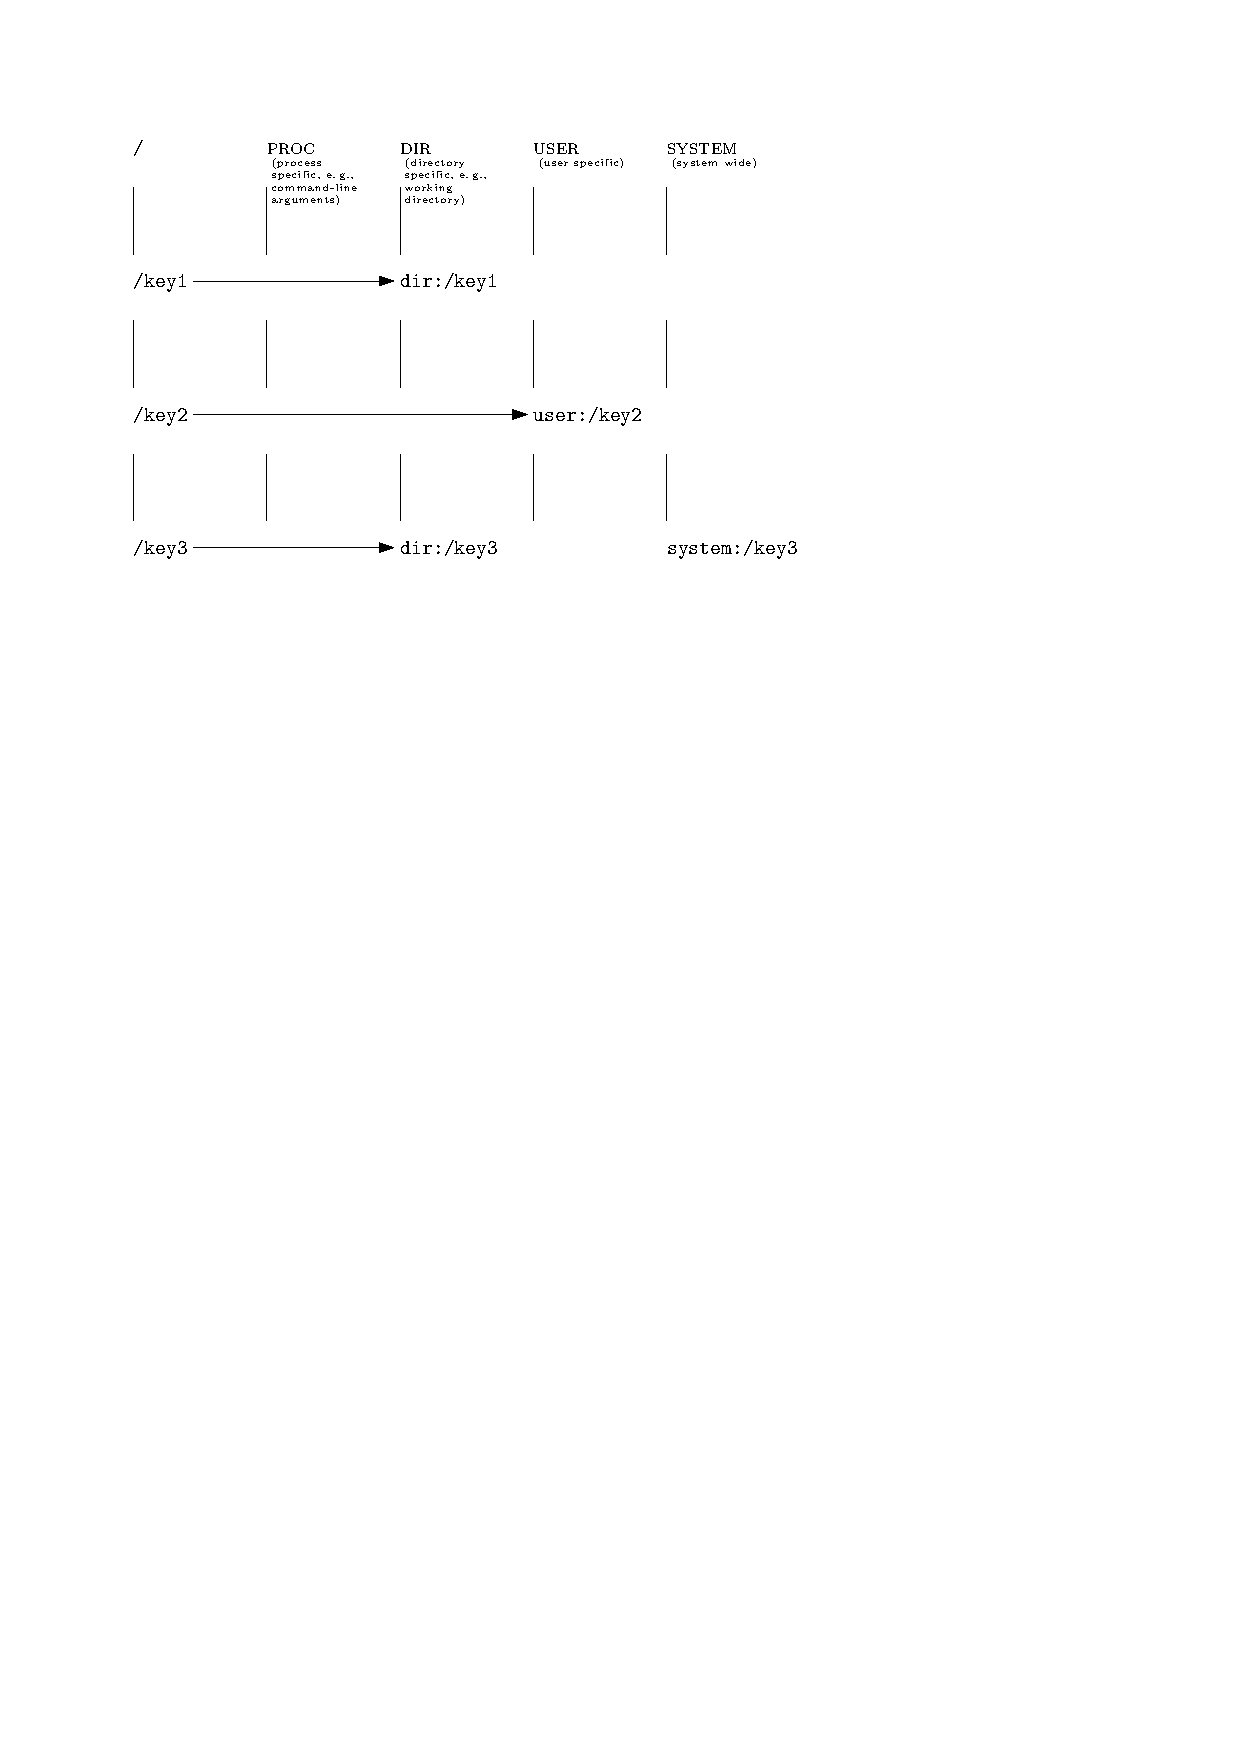
\includegraphics[scale=0.7]{cascading}
\end{frame}

\begin{frame}
	\frametitle{Contextual Values}

	\begin{task}
	What are contextual values?
	\end{task}

	\pause

	\ExecuteMetaData[../book/background.tex]{contextual-values}
\end{frame}

\begin{frame}
	\frametitle{Definition Context (Recapitulation)}

	\begin{task}
	What is context-aware configuration?
	\end{task}

	\pause

	\ExecuteMetaData[../book/background.tex]{context-definition}
\end{frame}

\begin{frame}
	\frametitle{Introspection vs.\ Code Generation (Recapitulation)}

	\begin{task}
	Advantages/Disadvantages of contextual values in key database?
	\end{task}

	\pause

	\begin{description} %[leftmargin=0cm] %TODO: move left
	\item[$+$] specification can be updated live on the system without recompilation
	\item[$+$] tooling has generic access to all specifications
 	\item[$+$] new features the key database (e.g., better validation) are immediately available consistently
	\item[$-$] less techniques for performance improvements
	\item[$-$] cannot be used if context differs within same thread
	\end{description}

	\begin{alertblock}{Implication}
	We generally prefer introspection, except for a very thin configuration access API.
	\end{alertblock}
\end{frame}

\begin{frame}
	\frametitle{Key Databases (Recapitulation)}

	\pause

	\methodQuestion{} \question{Which configuration systems/libraries/APIs have you already used or would like to use in one of your FLOSS project(s)?}

	\begin{itemize}
	\item Command-line arguments (\p{92}, $n=222$)
	\item environment variables (\p{79}, $n=218$)
	\item configuration files (\p{74}, $n=218$)
	\item Freedesktop standards (\p{20}, $n=205$)
	\item Windows Registry (\p{13}) ($\leq$ \p{13}, $n\geq185$) [talk later]
	\item X/Q/GSettings (\p{4}, \p{11}, \p{9})
	\item KConfig (\p{5})
	\item dconf (\p{7})
	\item plist (\p{7})
	\end{itemize}

\end{frame}

\begin{frame}
	\frametitle{Elektra (Recapitulation)}

	\pause

	\begin{itemize}
	\item is not only a key database but a specification language to describe a key database
	\item plugins implement the specification (could be distributed but focus is configuration files)
	\item is library based (no single point of failure, no distributed coordination needed)
	\item supports transactions (persisting whole KeySets at once)
	\item supports integration of existing configuration settings
	\end{itemize}
\end{frame}

%%%%%%%%%%%%%%%%%%%%%%%%%%%%%%%%%%%%%%%%%% 
\section{Terms and Properties}

\subsection{}

\begin{frame}
	\frametitle{Definition Configuration Management (Recapitulation)}

	\pause

	\begin{itemize}
	\item is a discipline in which configuration (in the broader sense) is administered.
	\item makes sure computers are assembled from desired parts and the correct applications are installed.
	\item has means to describe the desired configuration of the whole managed system.
	\item ensures that the execution environment of installed applications is as required.
	\end{itemize}
\end{frame}

\begin{frame}
	\frametitle{Possible Benefits of CM (Recapitulation)}

	\pause

	\begin{itemize} %[<+-| alert@+>]
	\item All advantages scripts have: \\
		Documentation, Customization, Reproducability
	\item Declarative description of the system \\
		(Infrastructure as Code~\cite{waldemar2013testing})
	\item Auditability
	\item Less configuration drift
	\item Error handling
	\item Pull/Push
	\item Reusability
	\item (Resource) Abstractions
	\end{itemize}
\end{frame}

\begin{frame}
	\frametitle{Infrastructure as Code}

	Once we described configuration settings,
	configuration settings are simply an instantiation of the configuration specifications.
	\vspace{1em}

	Code describing the instantiation is \textbf{CM code}.
	\vspace{1em}

	\textbf{Auditability:}
	Being informed about status and changes in the infrastructure.
	\vspace{1em}

	\begin{alertblock}{Goal}
	Single Source of Truth
	\end{alertblock}
\end{frame}

\begin{frame}
	\frametitle{Configuration Drift}

	Are derivations of the ``Single Source of Truth'' (the CM code).

	Caused by:

	\pause

	\begin{itemize}[<+-| alert@+>]
	\item manual configuration changes by administrators
	\item manual configuration changes by end users
	\item differences in updates (e.g., skipped or failed updates)
	\item failed attempts to change configuration
	\item applying different versions of CM code
	\item \dots
	\end{itemize}
\end{frame}

\begin{assignment}
	\begin{task}
	Break.
	\end{task}
\end{assignment}

\begin{frame}
	\frametitle{Push vs.\ Pull}

	\begin{itemize}[<+-| alert@+>]
	\item Push is more interactive.
	\item Push cannot do its job if nodes are not reachable.
	\item Push needs additional techniques to scale with many nodes.
	\item Push demands access to servers from a single server.
	\item Pull needs additional monitoring to know when a patch has been applied.
	\item Pull needs resources even if nothing is to do.
	\end{itemize}

	\begin{task}
	Do you prefer push or pull?
	What does your CM tool of choice use?
	\end{task}
\end{frame}


\begin{frame}
	\frametitle{Idempotence}

	idem + potence (same + power)
	\vspace{2em}

	Yield same result with any number of applications ($n\ge1$):
		
	\[
		f(f(x))=f(x)
	\]
\end{frame}


\begin{frame}
	\citet{wadler2003xml} describe two further properties:
	\vspace{2em}

	\begin{description}
	\item[Self-describing]
	means that from the configuration file alone we are able to derive the correct internal representation.

	\item[Round-tripping]
	means that if a data-structure (e.g., KeySet) is serialized and then parsed again, we end up with an identical internal representation.
	\end{description}

	\pause

	\vspace{2em}
	Round-tripping is a prerequisite of idempotence.

	\pause

	\begin{task}
	Explain the three concepts your neighbor (idempotence, self-describing, round-tripping).
	\end{task}
\end{frame}


%%%%%%%%%%%%%%%%%%%%%%%%%%%%%%%%%%%%%%%%%% 
\section{Validation}

\subsection{}

%Describe constraints in OOP (Babelsberg)?

\begin{frame}
	\frametitle{Goals}

	Checking the specifications vs.\ checking the settings.

\end{frame}

\begin{frame}
	\frametitle{Checking Configurations}

	Following properties of configuration settings can be checked:

	\begin{itemize}[<+-| alert@+>]
	\item structure
	\item values (data types)
	\item constraints
	\item semantic checks (e.g., IP, folder)
	\item domain-specific checks (e.g., databases)
	\item requirements (suitable configurations)
	\item context (context-aware configurations)
	\end{itemize}
\end{frame}

\begin{frame}[allowframebreaks]
	\frametitle{}
	\elektra{} supports many other data types, each implemented in its own plugin(s):
	\begin{description}
	\item [check/type] allows us to specify CORBA data types.
	Checking ``any'' (default) is always successful.
	The record and enum types defined by CORBA are not part of this plugin but of others as explained below.

	\item [check/enum] supports a list of supported values denoted by array indexes.
	\item [check/bool] transforms specific strings, for example ``true'' and ``false'', into the canonical boolean representation, i.\,e., ``0'' and ``1''.
	\item [check/ipaddr] checks if a string is a valid IP address.
	\item [check/path] checks presence, permissions, and type of paths in the file system.
	\item [check/date] supports to check date formats such as POSIX, ISO8601, and RFC2822.
	\item [check/validation] checks the configuration value with regular expressions.
	\item [check/condition] checks using conditionals and comparisons.
	\item [check/math] checks using mathematical expressions.
	\item [check/range] allows us to check if numerical values are within a range.
	\item [trigger/error] allows us to express unconditional failures.
	\end{description}
\end{frame}

\begin{frame}
	\frametitle{Checking Specifications}

	The goals of checking \elektra{Spec} are:

	\begin{itemize}[<+-| alert@+>]
	\item Defaults must be present for safe lookups.
	This goal also implies that there must be at least one valid configuration setting.
	\item Types of default values must be compatible with the types of the keys.
	\item Every contextual interpretation of a key must yield a compatible type.
	\item Links must not refer to each other in cycles.
	\item Every link and the pointee must have compatible types.
	\end{itemize}
\end{frame}

\begin{frame}[fragile]
	\frametitle{Example}

	\begin{code}[morekeywords={override},gobble=4]
	[sw/org/abc/has_true_arg]
	  type:=boolean
	  default:=0
	  override/#0:=/sw/org/abc/arg0
	  override/#1:=/sw/org/abc/arg1
	\end{code}
\end{frame}

\begin{frame}[fragile]
	\frametitle{Logfile Example}

	\begin{code}[morekeywords={path},gobble=4]
	[slapd/logfile]
	  check/path:=file
	\end{code}
\end{frame}

\begin{frame}[fragile]
	\frametitle{Logfile Extensions}

	\begin{code}[morekeywords={match,path},gobble=4]
	[slapd/logfile]
	  check/path:=file
	  check/validation:=^/var/log/
	  check/validation/message:=Policy violation:
	    log files must be below /var/log
	\end{code}
\end{frame}

\begin{frame}[fragile]
	\frametitle{Error Messages}

	Error messages are extremely important as they are the main communication channel to system administrators.\\
	Example specification:
	\vspace{1em}

	\begin{code}[morekeywords={assign,math},gobble=4]
	[a]
	  check/type:=long
	[b]
	  check/type:=long
	[c]
	  check/range:=0-10
	  assign/math:=../a+../b
	\end{code}
\end{frame}

\begin{frame}[fragile]
	\frametitle{Error Messages}

	Problems:
	\begin{itemize}[<+-| alert@+>]
	\item Generic vs.\ specific plugins
	\item General principles of good error messages~\cite{lee2011personifying}
	\item Give context
	\item Precisely locate the cause:
	\end{itemize}
	\vspace{1em}

	\pause[\thebeamerpauses]

	\begin{code}[language=CfgElektra,gobble=4]
	a=5  ; unmodified
	b=10 ; modification bit in metadata
	     ; is only set here
	c=15 ; unmodified by user but changed
	     ; later by assign/math
	\end{code}
\end{frame}

\begin{frame}[fragile]
	\frametitle{Example Error Messages}
\begin{verbatim}
Sorry, I was unable to change the configuration settings!
Description: I tried to set a value outside the range!
Reason: I tried to modify b to be 10 but this caused c to
        be outside of the allowed range (0-10).
Module: range
At: sourcefile.c:1234
Mountpoint: /test
Configfile: /etc/testfile.conf
\end{verbatim}
\end{frame}



%%%%%%%%%%%%%%%%%%%%%%%%%%%%%%%%%%%%%%%%%% 
\section{CM languages}

\subsection{}

\begin{frame}[fragile]
	\frametitle{Proteus (PCL)}
	\textsc{Proteus}~\cite{tryggeseth1995modelling} shows the tight relation between software configuration management, like Git or Svn, and configuration specification languages.
	\textsc{Proteus} (PCL) combines both worlds in a powerful build system.

	\begin{code}[basicstyle=\tiny,morekeywords={family,attributes,end,physical,default,classifications},gobble=4,language=]
	family CalcProg
		attributes
			HOME : string default "/home/ask/proteus/test";
			workspace := HOME ++ "/calc/src/"; // string concatenation
			repository := "calc/";
			end
		physical
			main => "main.C";
			defs => "defs.h";
			exe => "calc.x" attributes workspace := HOME ++ "/calc/bin"; end
			classifications status := standard.derived; end;
		end
	end
	\end{code}
\end{frame}

\begin{frame}
	\frametitle{NIX}

	The NIX language~\cite{dolstra2007purely} claims to be purely functional as a novel feature.
	The main concept is the referential transparency both for the configuration specification language and for the system itself.

	\textbf{Expressiveness:}
	NIX expressions, for example functions, describe how to build software packages.

	\textbf{Reasoning:}
	Because of the referential transparency of the system itself, every solution derived from the NIX expressions should be valid, so no reasoning or conflict handling is necessary.

	\textbf{Modularity:}
	The NIX expressions are modular because they ensure absence of side effects and thus can be easily composed.

	\textbf{Reusability:}
	Derivations that describe atomic build actions are reused in other derivations.
\end{frame}

\begin{frame}
	\frametitle{UML}
	\citet{felfernig1999knowledge,felfernig2000uml,felfernig2002joint} describe an approach where the unified modeling language (UML) is used as notation.

	\textbf{Expressiveness:}
	All UML features, including cardinality, domain-specific stereotypes and OCL-constraints are available.
	The basic structure of the system is specified using classes, generalization and aggregation.

	\textbf{Reasoning:}
	Customers provide additional input data and requirements for the actual variant of the product.

	\textbf{Modularity:}
	Generalization is present without multiple inheritance with disjunctive semantics, i.\,e., only one of the given subtypes will be instantiated.

	\textbf{Reusability:}
	For shared aggregation additional ports are defined for a part.
\end{frame}


\begin{frame}
	\frametitle{CFEngine}

	CFEngine~\cite{burgess2003theory,burgess1995cfengine,pandey2012investigating} is a language-based system administration tool that pioneered idempotent behavior.

	\textbf{Expressiveness:}
	CFEngine allows us to declare dependences and facilitates some high-level configuration specification constructs.
	In its initial variants it neither had validation specifications, cardinalities, nor higher-level relationships.

	\textbf{Reasoning:}
	Not supported.

	\textbf{Modularity:}
	Not supported.

	\textbf{Reusability:}
	Existing system administrator scripts can be profitably run from CFEngine.
\end{frame}



\begin{frame}
	\frametitle{Quattor (Pan)}

	\citet{cons2002pan} invented and used PAN for many machines within CERN.

	\textbf{Expressiveness:}
	The Pan language allows users to specify data types, validation with code snippets and constraints.
	The compiler uses a 5 step process: compilation, execution, insertions-of-defaults, validation, and serialization.

	\textbf{Reasoning:}
	Pan focuses on validating configurations, it is not able to generate new configurations.
	Pan provides type enforcement with embedded validation code.

	\textbf{Modularity:}
	The language has user-defined data types (called templates) but otherwise has only minimal support for modularity.

	\textbf{Reusability:}
	Reusability and collaboration is only possible via simple include statements and a simple inheritance mechanism of templates.
\end{frame}


\begin{frame}
	\frametitle{ConfValley (CPL)}

	\citet{huang2015confvalley} introduce systematic validation for cloud services.
	ConfValley uses a unified configuration settings representation for tens of different configuration file formats.

	\textbf{Expressiveness:}
	CPL is not able to specify dynamic and complex requirements.

	\textbf{Reasoning:}
	Constraints can be inferred by running an inference engine on configuration settings that are considered good (black-box approach).
	Within the validation engine, however, no constraint solver is available.

	\textbf{Modularity:}
	CPL aims at easy grouping of constraints.
	Adding language primitives need modifications in the compiler.

	\textbf{Reusability:}
	Using transformations and compositions, predicates can be reused in different contexts.
	Also with language constructs like \texttt{let}, specifications can be reused.
\end{frame}

%TODO: distributed vs. centralized

\begin{frame}
	\frametitle{Popular CMs today}

	\begin{itemize}[<+-| alert@+>]
	\item CFengine
	\item Bcfg2
	\item LCFG
	\item Config Mgmt
	\item Quattor
	\item Puppet
	\item Chef
	\item Ansible (Talk)
	\item SaltStack
	\item Rudder
	\item Spacewalk
	\end{itemize}
\end{frame}


\begin{frame}
	\frametitle{Conclusion}

	\begin{itemize}[<+-| alert@+>]
	\item Definition and challenges in configuration management.
	\item Properties: self-describing, idempotent, round-tripping.
	\item Validation is combined effort of devs and admins.
	\item Configuration management languages differ widely.
	\item Configuration specifications are always helpful.
	\end{itemize}
\end{frame}




%%%%%%%%%%%%%%%%%%%%%%%%%%%%%%%%%%%%%%%%%% 
\nocite{raab2017introducing}

\appendix

\begin{frame}[allowframebreaks]
	\bibliographystyle{plainnat}
	\bibliography{../shared/elektra.bib}
\end{frame}

\end{document}


%TODO: add cliffhanger with preview for next time
